\documentclass[conference]{IEEEtran}
\usepackage{amsmath, amssymb}
\usepackage{graphicx}
\usepackage{booktabs}
\usepackage{multirow}
\usepackage{array}
\usepackage{xcolor}
\usepackage[hidelinks]{hyperref}
\graphicspath{{../results/final/figures/}}
\setlength{\tabcolsep}{3.2pt}
\renewcommand{\arraystretch}{1.04}
\newcommand{\Log}{\mathrm{Log}}

\begin{document}

\title{Calibrated Confidence for Kilometre-Scale\\Feed-Forward SLAM}

\author{\IEEEauthorblockN{Kavish Vora \qquad Pranav Srivastava \qquad Mehrish Khan}
\IEEEauthorblockA{Mobile Robotics, Monsoon 2026, IIIT Hyderabad}}

\maketitle

\begin{abstract}
VGGT-Long runs the feed-forward model VGGT on overlapping windows of a long monocular drive and joins the windows in a
Sim(3) pose graph with equal edge weights. We asked whether VGGT's own per-pixel confidence, calibrated without any
training, gives better edge weights. Calibration works at the pixel level (calibration error 0.40 to 0.17 on held-out
LiDAR), and calibrated weights let a robust kernel keep the true loop closures of the hardest drive while it rejects
false ones, but on the eleven KITTI
odometry drives no weighting scheme changes the trajectory error by more than 3\%, even with weights computed from the
true errors. We show why: almost all of the error is in one number per seam, the relative scale, and that error is a
bias with one sign, which no variance weight can remove. VGGT stretches the first steps of every window and compresses
the last ones, so the map shrinks along the drive. We therefore calibrate the mean of the seam scale instead, with a
correction learned on other drives that needs no extra network inference. Inside VGGT-Long's own code at its chunk-30
setting, it lowers the mean trajectory error over the eleven drives from 44.70\,m to 28.09\,m (Wilcoxon $p=0.019$). At
chunk sizes 60 and 75 most drives still improve but the mean does not, because the bias that the correction removes is
much smaller there.
\end{abstract}

\section{Introduction}

Feed-forward 3D models such as VGGT \cite{vggt} return camera poses, depth, point maps and a per-pixel confidence for a
set of images in one forward pass. GPU memory limits one pass to a few dozen frames, so VGGT-Long \cite{vggtlong} cuts a
long drive into overlapping windows (\emph{chunks}), aligns neighbouring windows on their shared frames, adds loop
closures found by place recognition, and solves a Sim(3) pose graph. Every edge of that graph has the same weight,
although some edges are clearly worse than others and VGGT already reports how confident it is in every pixel.

Our hypothesis was that calibrated confidence makes better edge weights. This paper reports what we found when we
tested it on all eleven KITTI odometry drives with ground truth \cite{kitti}, and what follows from it:
\begin{itemize}
\item VGGT's confidence ranks pixel errors and can be calibrated on other drives (Sec.~\ref{sec:weights}). On the hardest
drive, calibrated edge weights let the robust kernel DCS \cite{dcs} keep the true loops while it rejects false ones. But they do
not change the trajectory error: all weighting schemes, including one built from the true edge errors, stay within 3\%
of equal weights.
\item The reason (Sec.~\ref{sec:why}): replacing each component of every seam by its true value shows that the scale
carries almost all of the error, and the scale error has the same sign on every drive. We measure the cause inside the
windows against ground truth: VGGT's early steps are too long and its late steps too short. For a bias of one sign,
equal weights are close to optimal and variance weights can only redistribute it; we show this with a simulation fed
with the measured errors of each drive.
\item The fix (Sec.~\ref{sec:method}): calibrate the \emph{mean} of the seam scale with the same tools, a fused scale
estimate and an isotonic curve, fitted leave-one-drive-out. It adds no network inference and 30 lines to VGGT-Long.
\item Results (Sec.~\ref{sec:results}): at chunk 30 the correction lowers the mean error of VGGT-Long's own code by 37\%
on eleven drives (8 better, 2 worse, $p=0.019$). We also report where it does not help (chunks 60 and 75) and why.
\end{itemize}

\section{Related work}

\textbf{Feed-forward reconstruction of long sequences.} DUSt3R \cite{dust3r} and MASt3R \cite{mast3r} regress point maps
with confidence for image pairs; VGGT \cite{vggt} handles many views and predicts cameras, relative to its first input
frame. VGGT-Long \cite{vggtlong} chunks long drives and joins the chunks with confidence-weighted Sim(3) alignment, SALAD
\cite{salad} loop retrieval and an equal-weight Sim(3) pose graph. VGGT-SLAM \cite{vggtslam} and VGGT-SLAM~2.0
\cite{vggtslam2} build submap graphs; the latter notes that the first frame of a submap ``is also unequally
influential''. $\pi^3$ \cite{pi3} removes the fixed reference view, which ``can lead to instability and failures if the
reference is suboptimal''. MASt3R-SLAM \cite{mast3rslam} is a dense SLAM system on MASt3R.

\textbf{Scale drift in chunked feed-forward SLAM.} Sim(3) graphs for monocular scale drift go back to Strasdat et
al.~\cite{strasdat}. Several recent works report that chunked VGGT pipelines shrink the map. VGGT-Bridge \cite{bridge}
measures the Umeyama scale of every sequential seam (mean $\log s=-0.037$ on KITTI, ``roughly 3.6\% smaller scale than
its predecessor''), attributes it to VGGT anchoring each chunk at its first frame, shows that the sign flips for coarse
chunks fed in reverse order, and adds reversed coarse chunks as skip edges (on drive 08 this raises the network inference time of its base system
from 197.6\,s to 307.9\,s). VGGT-Align
\cite{align} reports that VGGT-Long's scale drops to ``approximately 0.5'' on drive 08, calls it ``compounding bias rather
than zero-mean noise'', and replaces the seam scale with a road-plane scale. VGGT-Motion \cite{motion} observes ``a
systematic bias at submap boundaries'', AMB3R-SLAM \cite{amb3r} uses the middle frame of each submap as reference, and
LongStream \cite{longstream} names ``reference and scale biases''. We build on these observations; what we add is the
oracle breakdown, the measurement inside the windows, the explanation of why edge weighting cannot help, and a
correction learned from data that needs neither extra inference nor a road.

\textbf{Confidence and calibration.} Confidence heads are trained with a loss of the form $Ce-\alpha\log C$ \cite{kendall}.
The audit of Deng et al.~\cite{audit} finds the confidence of seven feed-forward models off ``by at least 2.4$\times$''
and proposes a power-law correction; Srinivasan and Nordstr\"om \cite{knows} show that VGGT's point-map confidence
predicts pose failure worse than a probe on its features (ROC-AUC 79.7\% against 93.5\%); GeoCond \cite{geocond} learns
pose-level reliability for graph weighting. We calibrate with isotonic regression \cite{kuleshov}. Dynamic Covariance
Scaling (DCS) \cite{dcs} protects pose graphs against false loops.

\section{Setup}
\label{sec:setup}

\textbf{Pipeline.} A drive is cut into windows of $W$ frames that overlap by $O$ (written $W/O$). For two neighbouring
windows $i,j$, VGGT-Long estimates $Z_{ij}=(s,R,t)\in\mathrm{Sim}(3)$ from the point maps of the shared frames
(confidence-weighted, Huber IRLS, scale as a ratio of weighted spreads). Loop windows join revisits found by SALAD. The
trajectory is
\begin{equation}
\{S_k^\star\}=\arg\min_{\{S_k\}}\sum_{(i,j)}r_{ij}^\top\Lambda_{ij}r_{ij},
\label{eq:graph}
\end{equation}
where $r_{ij}=\Log(Z_{ij}^{-1}S_i^{-1}S_j)\in\mathbb{R}^7$ and $\Lambda_{ij}=I$ in VGGT-Long. We re-implemented the
back end so that $\Lambda_{ij}$ can be changed; with equal weights it agrees with the original code within 2.4\% ATE on
every drive but one (Sec.~\ref{sec:results}), which also reports runs of VGGT-Long's own code.

\textbf{True edge errors.} For each window $k$ we fit a Sim(3) gauge $A_k$ that maps its predicted cameras onto the
ground-truth cameras. The true error of an edge is $e_{ij}=\Log(Z_{ij}^{-1}A_i^{-1}A_j)$: three rotation, three
translation and one log-scale component. A positive log-scale error means VGGT-Long's seam scale is too small, so the
map shrinks. Windows in which the car hardly moves are skipped.

\textbf{Data and metrics.} KITTI odometry drives 00 to 10 (23{,}201 frames, 22\,km), colour camera. We score with ATE
after Sim(3) alignment \cite{umeyama} and report the KITTI relative translation error $t_\mathrm{rel}$ as a second
metric. KITTI's ground truth is inconsistent in height where a street is revisited, as SemanticKITTI reports
\cite{semkitti} (``streets that are revisited after some time have different height''); against SemanticKITTI's poses,
the ground-truth gap at revisits reaches 4.4\,m on 02, 6.1\,m on 08 and 3.3\,m on 09. All methods are scored against the
same ground truth.

\textbf{Protocol.} The analyses that need LiDAR or many solves per drive (pixel calibration, seam error prediction,
false loops; Sec.~\ref{sec:weights}) use drives 00, 02, 05 and 07: everything is fitted on 05 and 07 and tested on 00
and 02. Everything else is fitted on the other ten drives and applied to the held-out drive (leave one drive out),
including the edge weights of Table~\ref{tab:weights} and every scale correction. The evaluation at 60/30 and 75/30 was fixed before
those runs. We compare paired per-drive results with the Wilcoxon
signed-rank test and give a bootstrap 95\% interval of the change of the mean.

\textbf{Baseline check.} VGGT-Long's own code at 30/15 gives a mean ATE of 44.70\,m over the eleven drives; the paper
reports 44.713\,m for chunk 30 \cite{vggtlong}, and every drive agrees within 1.3\%. All runs use one RTX~A4000 (16\,GB)
in bfloat16.

\begin{figure*}[t]
\centering
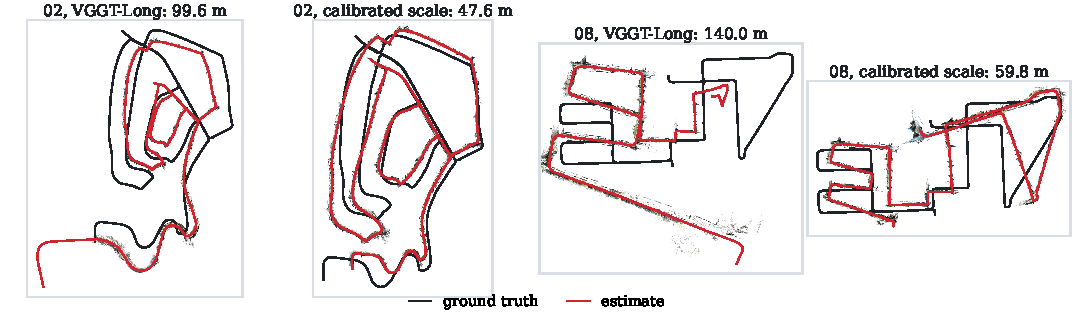
\includegraphics[width=\textwidth]{report_maps.pdf}
\caption{VGGT-Long's own code at 30/15 on drives 02 and 08, without and with the calibrated seam scale: point maps and
trajectories after Sim(3) alignment to the ground truth (top view). Without the correction the map shrinks along the
drive, and loop closure cannot pull the long middle sections into place.}
\label{fig:maps}
\end{figure*}

\section{Calibrated confidence as edge weights}
\label{sec:weights}

\textbf{Pixels.} Against 478 million LiDAR pixels of drives 00, 02, 05 and 07 (window 30/15), the error of VGGT's depth falls with
confidence, but more slowly than $1/C$ (log-log slope $-0.71$ on 00 and 02, Spearman $-0.34$). An isotonic map from
confidence to expected squared error, fitted on 05 and 07, reduces the calibration error on 00 and 02 from 0.40 (raw)
and 0.25 (power law of \cite{audit}) to 0.17 (point head: 0.58, 0.52, 0.31).

\textbf{Edges.} A seam's mean confidence ranks its rotation error (Spearman $-0.42$ on 607 held-out seams of 00 and 02)
but hardly its translation error ($-0.15$); the alignment residual ranks translation better ($0.53$). Calibrated block
variances predict the size of seam errors within a factor of 1.5.

\textbf{Trajectories.} Table~\ref{tab:weights} compares six weightings at 30/15 on all eleven drives, each fitted on the
other drives: equal weights, one variance per block (uniform), raw confidence, an isotonic map of the alignment
residual (geometry), our calibrated confidence, and an oracle that uses each edge's true error. All six lie within
44.38 to 45.66\,m, less than 3\% apart. Loop closure, by contrast, cuts the error by 41\% (chain without loops:
77.48\,m).

\begin{table}[t]
\centering
\caption{Mean ATE (m) over 11 drives at 30/15 for six edge weightings, with the measured seam scales, with the scale
corrected by our method (Sec.~\ref{sec:method}), and with the true seam scale.}
\label{tab:weights}
\footnotesize
\begin{tabular}{lcccccc}
\toprule
Seam scale & equal & uniform & raw conf. & geometry & calibrated & oracle \\
\midrule
measured & 45.66 & 45.24 & 44.85 & 44.61 & 44.73 & 44.38 \\
corrected (C4) & 28.17 & 27.33 & 26.92 & 27.31 & 26.48 & 27.28 \\
true & 14.47 & 22.81 & 24.47 & 14.46 & 14.12 & 52.09 \\
\bottomrule
\end{tabular}
\end{table}

\textbf{False loops.} Weights do matter when loops are wrong. We added 1 to 16 false loops between windows at least 50\,m
apart (20 seeds, drives 00, 02, 05, 07, window 30/15), each with the weight of the most trusted true loop. Without a robust kernel or
with Huber, one false loop breaks every scheme. With DCS at the threshold tuned on 05 and 07, equal weights fail with a
single false loop on every drive; in a sweep of the threshold from $10^{-6}$ to $10^3$, the best value lets them survive
one or two false loops on 00, 02 and 05 but none on 07, because the residuals of true and false loops are not measured
against any uncertainty. With fitted variances DCS survives more false loops on some drives (up to 8 on 00), but on 02
most weighted schemes then make DCS discard the true loops of the clean graph as well (ATE 174 to 189\,m instead of 114
to 122\,m). Calibrated confidence is the only weighting with which DCS keeps 02's true loops (118.6\,m) and still
rejects up to four false ones there; on 00 and 05 it survives one, on 07 none. No scheme survives on all four drives
(appendix, Fig.~\ref{fig:stress}).



\begin{table*}[t]
\centering
\caption{ATE (m) at 30/15 with loop closure. Upstream: VGGT-Long's released code, without and with the 30-line patch.
Ours: our back end. Every correction is fitted on the other ten drives. Nested: for each drive, the variant chosen by an
inner leave-one-out on the other drives (C4 for ten drives, C1 for 01). True scale: every seam scale replaced by its
true value (bound).}
\label{tab:main}
\footnotesize
\begin{tabular}{llrrrrrrrrrrrr}
\toprule
& & 00 & 01 & 02 & 03 & 04 & 05 & 06 & 07 & 08 & 09 & 10 & mean \\
\midrule
\multirow{2}{*}{Upstream} & VGGT-Long & 9.07 & 96.33 & 99.65 & 19.53 & 11.22 & 10.24 & 10.15 & 3.98 & 140.03 & 50.64 & 40.86 & 44.70 \\
& + calibrated scale (C4) & 10.43 & 77.16 & 47.62 & 18.04 & 5.65 & 7.19 & 5.81 & 4.40 & 59.82 & 50.49 & 22.37 & \textbf{28.09} \\
\midrule
\multirow{5}{*}{Ours} & VGGT-Long (equal weights) & 9.02 & 96.40 & 110.18 & 19.71 & 11.21 & 10.00 & 9.94 & 3.98 & 140.54 & 50.35 & 40.96 & 45.66 \\
& + constant (C1) & 9.03 & 156.67 & 67.81 & 6.87 & 7.88 & 9.64 & 8.95 & 3.82 & 64.18 & 50.57 & 23.37 & 37.16 \\
& + calibrated scale (C4) & 10.48 & 77.64 & 48.29 & 18.10 & 5.61 & 7.04 & 5.81 & 4.37 & 59.82 & 50.29 & 22.39 & \textbf{28.17} \\
& + nested choice & 10.48 & 156.67 & 48.29 & 18.10 & 5.61 & 7.04 & 5.81 & 4.37 & 59.82 & 50.29 & 22.39 & 35.35 \\
& true scale & 6.57 & 42.62 & 29.38 & 2.95 & 1.00 & 3.70 & 3.21 & 2.35 & 40.37 & 18.67 & 8.31 & 14.47 \\
\bottomrule
\end{tabular}
\end{table*}

\section{Why edge weights cannot help}
\label{sec:why}

\textbf{The error is in the scale.} We replace one component of every seam by its true value and solve again
(Table~\ref{tab:oracle}). True rotations change the mean ATE at 30/15 by 4\%, true translations not at all; true scales
cut it by 68\% (45.66 to 14.76\,m), and true rotation and scale together by 91\%. The same holds at 60/30 and 75/30.

\begin{table}[t]
\centering
\caption{Mean ATE (m), 11 drives, when one component of every seam is replaced by its true value. Here the true
value replaces the error component in the Lie algebra; the true-scale rows of Tables~\ref{tab:weights} and
\ref{tab:main} rescale each seam about its overlap cameras as the method does (Eq.~\ref{eq:correct}), hence 14.76
against 14.47\,m at 30/15.}
\label{tab:oracle}
\footnotesize
\begin{tabular}{lcccccc}
\toprule
Setting & measured & rot. & trans. & scale & rot.+scale & all \\
\midrule
30/15, loops & 45.66 & 43.80 & 45.74 & 14.76 & 4.15 & 1.53 \\
30/15, no loops & 77.48 & 71.99 & 77.76 & 32.29 & 6.84 & 1.26 \\
60/30, loops & 25.82 & 23.51 & 25.56 & 14.79 & 4.99 & 2.63 \\
75/30, loops & 24.61 & 22.12 & 24.43 & 15.27 & 5.14 & 2.95 \\
\bottomrule
\end{tabular}
\end{table}

\textbf{The scale error is a bias.} At 30/15 the mean seam log-scale error is positive on all eleven drives (+0.006 to
+0.046; pooled $+0.0136\pm0.0019$ over 1{,}510 seams). Summed along a drive without loops, it shrinks the map by a
factor of 17.6 on average, and by 77 on drive 02. Fig.~\ref{fig:mech}a shows where it comes from: we compare each
predicted step inside a window with the true step. Steps early in a window are up to about 8\% too long and late steps about
2.5\% too short (median ratio of the first to the second half: 1.042), with the same shape at all three window sizes. A seam
compares the late part of one window with the early part of the next, so its scale is too small. The bias grows with
how far the car moves within a window relative to the scene depth (Fig.~\ref{fig:mech}b): at 30/15 from about $+0.01$
for the slowest fifth of seams to $+0.027$ for the fastest.

\begin{figure}[t]
\centering
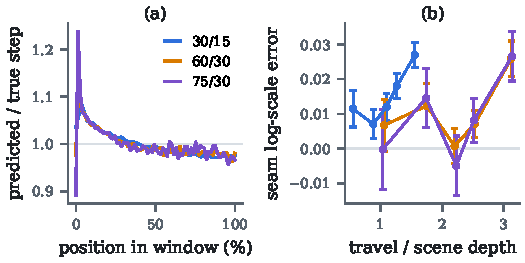
\includegraphics[width=\columnwidth]{report_mechanism.pdf}
\caption{(a) Predicted step divided by true step, by position in the window (geometric mean over 1{,}410, 674 and 433
windows of 11 drives). (b) Seam log-scale error (true over measured) against the car's travel in the overlap divided by
the median scene depth, five equal groups of seams per setting, mean $\pm$ standard error.}
\label{fig:mech}
\end{figure}

\textbf{Weights redistribute; they do not remove.} On a chain closed by one loop, least squares spreads the loop's
mismatch over the seams in proportion to their variances. For zero-mean noise, the extra error variance of equal over
perfect weights at node $m$ of $N$ is $V(m/N-V_m/V)^2$, where $V_m$ is the summed variance of the first $m$ seams and
$V$ the total: it is small unless the noisy seams sit together. A bias adds the same error to every seam, which equal
weights spread evenly and correctly, while variance weights push it onto the noisy seams. We simulated one loop per
drive with that drive's measured noise profile and bias (2{,}000 draws): without the bias, perfect variance weights
would gain at most 5.8\% (drive 03); with the measured bias they are worse than equal weights by more than 2\% on seven
of eleven drives (up to 21\%, drive 04). This is why the weightings in Table~\ref{tab:weights} cannot separate: they
act on the variance while the error is in the mean. The other rows of Table~\ref{tab:weights} agree. With the true
scale, calibrated weights are the best of the six (14.12\,m). With our corrected scale they give 26.48 against
28.17\,m for equal weights, but they are better on only five drives, worse on 02 and unchanged on the five drives
without loops, so we do not claim a gain from them. The oracle with the true scale (52.09\,m) is an artefact: every
seam's true scale error is then zero, its oracle variance falls to the numerical floor, and the solve becomes
ill-conditioned.

\begin{figure*}[t]
\centering
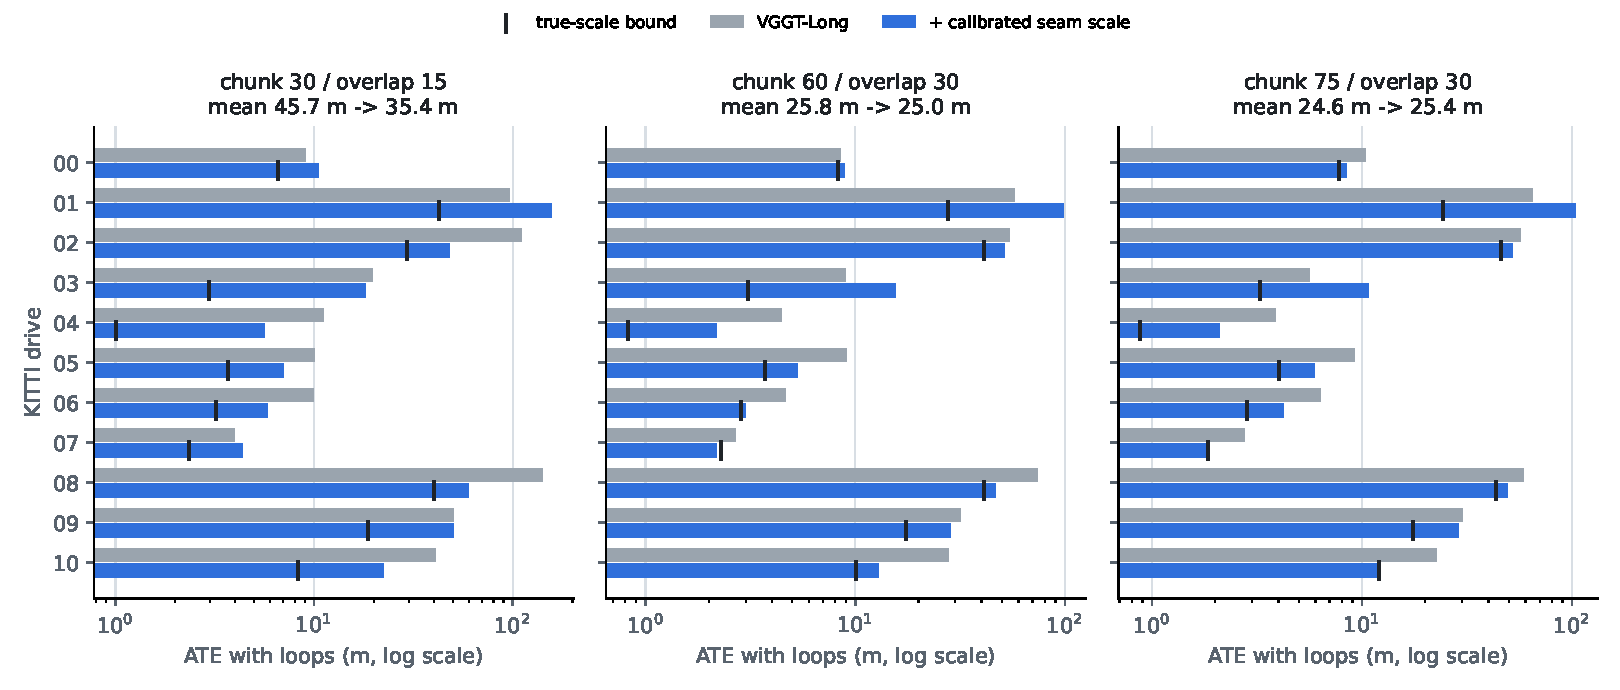
\includegraphics[width=0.92\textwidth]{fig_ate.pdf}
\caption{ATE with loop closure per drive in our back end at three window settings (log scale): VGGT-Long, VGGT-Long with
the calibrated seam scale (C4), and the true-scale bound.}
\label{fig:ate}
\end{figure*}

\section{Calibrated seam scale}
\label{sec:method}

The previous section points to calibrating the \emph{mean} of the seam scale. We keep VGGT-Long unchanged except for one
number per seam. For a seam with estimate $(s,R,t)$ mapping window $j$ into window $i$,
\begin{equation}
\log s' = \log s + c,\qquad t' = t + (s-s')\,R\,\bar m_j,
\label{eq:correct}
\end{equation}
where $\bar m_j$ is the mean camera centre of window $j$'s shared frames, which therefore keeps its image. Loop edges and
edge weights are unchanged. The correction $c$ uses two quantities that both windows already provide:
\begin{itemize}
\item $x_1$, a second scale estimate: for each shared frame, the median over confident pixels of $\log(d_i/d_j)$, the
ratio of the two windows' depth-head predictions of the same pixel; $x_1$ is the median over frames minus $\log s$.
\item $x_2=\log(L_j/D_j)$, the path length of window $j$'s shared cameras over the median depth of its points: the
travel per window of Fig.~\ref{fig:mech}b.
\end{itemize}
The correction has two calibrated stages, both fitted on the seams of the other drives against the true log-scale error
$y$:
\begin{equation}
c = \underbrace{a + b\,x_1}_{\text{fusion}} + \underbrace{g(x_2)}_{\text{isotonic curve}},
\end{equation}
where $a,b$ come from a ridge regression of $y$ on $x_1$, and $g$ is an isotonic regression \cite{kuleshov} of the
remaining error on $x_2$, the same tool we used to calibrate pixel confidence. Where a feature is undefined (fewer than
four usable frames, or a car that hardly moves) its term falls back to the mean of $y$ or to zero. We call this C4; C1
is the constant $c=\bar y$ alone. The patch to \texttt{vggt\_long.py} computes $x_1$ and $x_2$ from the chunk files that
VGGT-Long already saves; it applies exactly the corrections of our pipeline (72 of 72 seams on drive 07 at 30/15,
correlation 1.000), and plain and patched runs perform the same chunk inferences and alignments.

\section{Results}
\label{sec:results}





\textbf{Main result.} Table~\ref{tab:main}, Fig.~\ref{fig:maps}, and all drives in the appendix (Fig.~\ref{fig:traj}). In VGGT-Long's own code at 30/15, the calibrated seam
scale lowers the mean ATE over the eleven drives from 44.70\,m to 28.09\,m ($-37.2\%$; geometric mean of the per-drive
ratios 0.704). Eight drives improve, 09 is unchanged, and two get worse: 00 (9.07 to 10.43\,m) and 07 (3.98 to
4.40\,m). The paired test gives $p=0.019$ and the bootstrap interval of the change of the mean is $[-51\%,-15\%]$. The
gain is carried by the long drives with strong drift (02: 99.65 to 47.62\,m, 08: 140.03 to 59.82\,m); without these two,
the mean still falls by 20\% (28.00 to 22.39\,m), while the median moves little (19.53 to 18.04\,m) because the short
drives were already accurate. Our back end gives the same picture (45.66 to 28.17\,m, $p=0.019$); the two pipelines
agree within 2.4\% on every run except plain 02 (99.65 against 110.18\,m). The KITTI relative error $t_\mathrm{rel}$
falls by 37\% as well (15.84\% to 9.99\% in VGGT-Long's code), and the rotation error $r_\mathrm{rel}$ by 4\%: the
correction acts on scale only.

\textbf{Choice of variant.} When the variant itself is chosen by an inner leave-one-out (nested row), it picks C4 for ten
drives and C1 for drive 01, where the constant over-corrects (156.67\,m). The nested result, 35.35\,m ($-22.6\%$,
$p=0.083$), is the conservative estimate of what selecting among our variants yields; C4 was fixed as the method for
VGGT-Long's code before those runs.



\textbf{Larger chunks.} Table~\ref{tab:chunks}, Fig.~\ref{fig:ate}, and per-drive values in the appendix
(Table~\ref{tab:big}). At 60/30 and 75/30, eight of eleven drives still improve with C4, but 01 and 03 get clearly worse
(75/30: $\times$1.42 and $\times$2.16) and the mean changes by only $-6.2\%$ and $-2.5\%$ ($p=0.18$ and $0.28$). The
bias that the correction removes is much smaller there: per frame of window step it falls from $+0.00091$ at 30/15 to
$+0.00019$ at 75/30, and the drift without loops from $\times$17.6 to $\times$1.7. At 75/30 the drive means range from
$-0.006$ to $+0.032$, with 01, 03 and 05 at or below zero, so a correction learned on other drives can point the wrong
way, and Fig.~\ref{fig:mech}b shows no clean dependence on travel. The remaining scale error at large chunks is mostly
random from seam to seam; a calibration of the mean cannot remove it, although the true-scale bound is still about
15\,m at every setting. In VGGT-Long's code at 75/30 we checked agreement on five drives (03, 04, 06, 07, 10): the patch
changes ATE in the same direction as in our pipeline on all five. Coefficients do not transfer between settings: C4
fitted at 30/15 and applied at 60/30 gives 71.60\,m.

\begin{table}[t]
\centering
\caption{Our back end at three window settings, 11 drives, loops on. Bias: pooled seam log-scale error; drift: mean
factor by which the map shrinks without loops. Changes are of the mean ATE against VGGT-Long.}
\label{tab:chunks}
\footnotesize
\begin{tabular}{lccc}
\toprule
& 30/15 & 60/30 & 75/30 \\
\midrule
Seam bias & +0.0136 & +0.0102 & +0.0086 \\
\quad standard error & 0.0019 & 0.0026 & 0.0039 \\
Bias per frame of step & +0.00091 & +0.00034 & +0.00019 \\
Drift without loops & $\times$17.6 & $\times$2.4 & $\times$1.7 \\
\midrule
VGGT-Long ATE (m) & 45.66 & 25.82 & 24.61 \\
C1 constant & $-18.6\%$ & $-7.1\%$ & $-2.1\%$ \\
C4 calibrated scale & $\mathbf{-38.3\%}$ & $-6.2\%$ & $-2.5\%$ \\
\quad drives better / worse & 8 / 2 & 8 / 3 & 8 / 3 \\
\quad Wilcoxon $p$ & 0.019 & 0.175 & 0.278 \\
$t_\mathrm{rel}$ with C4 & $-37\%$ & $-10\%$ & $-7\%$ \\
True scale (bound) & $-68\%$ & $-44\%$ & $-40\%$ \\
\bottomrule
\end{tabular}
\end{table}

\textbf{Without loop closure.} At 30/15 VGGT-Long's map ends 26 to 55 times too small on the three longest drives
(00, 02, 08). With the correction, 00 and 08 end within a factor of 1.9 of the true scale, but 02 overshoots and ends
24 times too large, and on 01, 03 and 06 the end scale moves away from the true one. The chain ATE falls
by 17\% with C4 (77.48 to 64.51\,m), less than with loops, because the remaining error has one sign along a drive and
adds up where no loop removes it (appendix, Fig.~\ref{fig:drift}).



\textbf{Reference frame.} If the bias came only from the first-frame reference, moving the reference to the middle of
the window should reduce it. At 30/15 it does the opposite: the pooled bias rises from $+0.0136$ to $+0.0218$, larger on
11 of 11 drives, and the mean ATE rises from 45.66 to 52.43\,m (without loops 77.48 to 95.17\,m). The in-window profile
keeps its shape for any reference; only the steps next to the reference change.

\textbf{Context.} MASt3R-SLAM \cite{mast3rslam} (our run of the released code, checked on TUM fr1/desk, where it gives
0.016\,m as in its paper) loses tracking on all four drives we ran (00, 02, 05, 07; 6\% to 45\% of the path tracked), as
VGGT-Long reports. Larger chunks are still more accurate than calibrated small ones: plain VGGT-Long at 75/30 gives
24.61\,m in our runs, and the paper reports 26.36\,m and 22.72\,m for chunks 60 and 90 \cite{vggtlong}. Calibration
offers a smaller error at the 30-frame chunk, with 9.5\,GB peak GPU memory instead of 13.1\,GB at 75/30, not a better
result than large chunks.

\section{Conclusion}

Calibrated pixel confidence is a useful signal for VGGT-Long, but not as an edge weight for accuracy: on its pose graph
the error that matters is a bias in the seam scale, which variance weights cannot remove. As a weight, its clearest
use is robustness: with it, DCS keeps the true loops of the hardest drive and rejects false ones there, where equal
weights fail with a single false loop, although no weighting is robust on every drive. Calibrating the mean of the
seam scale, learned on other drives and without extra inference, lowers VGGT-Long's error by 37\% at chunk 30 in its
own code, and at larger chunks, where the bias is small, it helps most drives but not the mean.

\section{Limitations and future work}

All results are on one dataset, eleven drives of KITTI, and the correction is fitted on drives from the same car and
camera; it may not transfer to other cameras, scenes or speeds, and its coefficients must be refitted for each window
setting. Its form (which features, fusion and curve) was chosen on these same drives; the coefficients never see the
drive they correct, but a test on drives not used for any choice would be stronger. With eleven drives the statistics are limited, and two drives get worse even where
the mean improves. The ground truth is inconsistent in height at revisits of 02, 08 and 09, which affects all methods
equally but limits what loop-closed ATE can measure there. Our edge labels come from fitting window gauges to GPS/INS
poses, not from an independent sensor. We did not test other feed-forward models, such as $\pi^3$, which has no
reference frame and may not show the in-window profile.

Three directions follow. First, a lower-noise estimate of the seam scale, for example weighting the alignment points by
depth, is what larger chunks would need, since their remaining error is random rather than a bias. Second, the
correction should be tested on a second driving dataset with exact ground truth, such as Virtual KITTI 2 or Waymo, and
on non-driving data. Third, the cause of the in-window profile itself, which does not follow the reference frame in our
measurements, deserves a direct study inside the model.

\begin{thebibliography}{99}
\footnotesize
\bibitem{vggt} J.~Wang, M.~Chen, N.~Karaev, A.~Vedaldi, C.~Rupprecht, and D.~Novotny, ``VGGT: Visual geometry grounded
transformer,'' in \emph{Proc. CVPR}, 2025.
\bibitem{vggtlong} K.~Deng, Z.~Ti, J.~Xu, J.~Yang, and J.~Xie, ``VGGT-Long: Chunk it, loop it, align it, pushing VGGT's
limits on kilometer-scale long RGB sequences,'' in \emph{Proc. ICRA}, 2026. arXiv:2507.16443v2.
\bibitem{kitti} A.~Geiger, P.~Lenz, and R.~Urtasun, ``Are we ready for autonomous driving? The KITTI vision benchmark
suite,'' in \emph{Proc. CVPR}, 2012.
\bibitem{dcs} P.~Agarwal, G.~D.~Tipaldi, L.~Spinello, C.~Stachniss, and W.~Burgard, ``Robust map optimization using dynamic
covariance scaling,'' in \emph{Proc. ICRA}, 2013.
\bibitem{dust3r} S.~Wang, V.~Leroy, Y.~Cabon, B.~Chidlovskii, and J.~Revaud, ``DUSt3R: Geometric 3D vision made easy,'' in
\emph{Proc. CVPR}, 2024.
\bibitem{mast3r} V.~Leroy, Y.~Cabon, and J.~Revaud, ``Grounding image matching in 3D with MASt3R,'' in \emph{Proc. ECCV},
2024.
\bibitem{salad} S.~Izquierdo and J.~Civera, ``Optimal transport aggregation for visual place recognition,'' in \emph{Proc.
CVPR}, 2024.
\bibitem{vggtslam} D.~Maggio, H.~Lim, and L.~Carlone, ``VGGT-SLAM: Dense RGB SLAM optimized on the SL(4) manifold,'' in
\emph{Proc. NeurIPS}, 2025.
\bibitem{vggtslam2} D.~Maggio and L.~Carlone, ``VGGT-SLAM 2.0: Real-time dense feed-forward scene reconstruction,''
arXiv:2601.19887, 2026.
\bibitem{pi3} Y.~Wang \emph{et al.}, ``$\pi^3$: Permutation-equivariant visual geometry learning,'' in \emph{Proc. ICLR},
2026. arXiv:2507.13347.
\bibitem{mast3rslam} R.~Murai, E.~Dexheimer, and A.~J.~Davison, ``MASt3R-SLAM: Real-time dense SLAM with 3D reconstruction
priors,'' in \emph{Proc. CVPR}, 2025.
\bibitem{strasdat} H.~Strasdat, J.~M.~M.~Montiel, and A.~J.~Davison, ``Scale drift-aware large scale monocular SLAM,'' in
\emph{Proc. RSS}, 2010.
\bibitem{bridge} S.~Choi, H.~Bae, S.~Baek, and J.~Kim, ``VGGT-Bridge: Beyond sequential pose graphs via coarse-stride skip
edges,'' in \emph{Proc. ACCV}, 2026. arXiv:2610.06594v2.
\bibitem{align} W.~Zhang \emph{et al.}, ``VGGT-Align: Bridging local reconstruction and global consistency for
long-sequence 3D reconstruction,'' in \emph{Proc. ACM MM}, 2026. arXiv:2608.15260.
\bibitem{motion} Z.~Xiong, C.~Zhang, Q.~Xu, and W.~Tao, ``VGGT-Motion: Motion-aware calibration-free monocular SLAM for
long-range consistency,'' arXiv:2602.05508, 2026.
\bibitem{amb3r} H.~Wang and L.~Agapito, ``AMB3R-SLAM: Kilometer-scale SLAM with hierarchical backend,'' arXiv:2609.19518,
2026.
\bibitem{longstream} C.~Cheng \emph{et al.}, ``LongStream: Long-sequence streaming autoregressive visual geometry,''
arXiv:2602.13172, 2026.
\bibitem{kendall} A.~Kendall and Y.~Gal, ``What uncertainties do we need in Bayesian deep learning for computer vision?,''
in \emph{Proc. NeurIPS}, 2017.
\bibitem{audit} N.~N.~Deng, Q.~Cheng, N.~Zeller, and D.~Cremers, ``A calibration audit of confidence in feed-forward 3D
reconstruction models,'' arXiv:2608.29705, 2026.
\bibitem{knows} A.~T.~Srinivasan and D.~Nordstr\"om, ``Does VGGT know what it does not know?,'' arXiv:2610.35806, 2026.
\bibitem{geocond} D.~Ahmedt-Aristizabal, M.~A.~Armin, R.~Tsuchida, and L.~Petersson, ``GeoCond: A conditioning-aware
reliability adapter for feed-forward 3D reconstruction,'' in \emph{Proc. WACV}, 2027. arXiv:2609.18465.
\bibitem{kuleshov} V.~Kuleshov, N.~Fenner, and S.~Ermon, ``Accurate uncertainties for deep learning using calibrated
regression,'' in \emph{Proc. ICML}, 2018.
\bibitem{umeyama} S.~Umeyama, ``Least-squares estimation of transformation parameters between two point patterns,''
\emph{IEEE TPAMI}, vol.~13, no.~4, pp.~376--380, 1991.
\bibitem{semkitti} J.~Behley, M.~Garbade, A.~Milioto, J.~Quenzel, S.~Behnke, C.~Stachniss, and J.~Gall,
``SemanticKITTI: A dataset for semantic scene understanding of LiDAR sequences,'' in \emph{Proc. ICCV}, 2019.
\end{thebibliography}

\onecolumn
\appendix

\begin{figure}[!h]
\centering
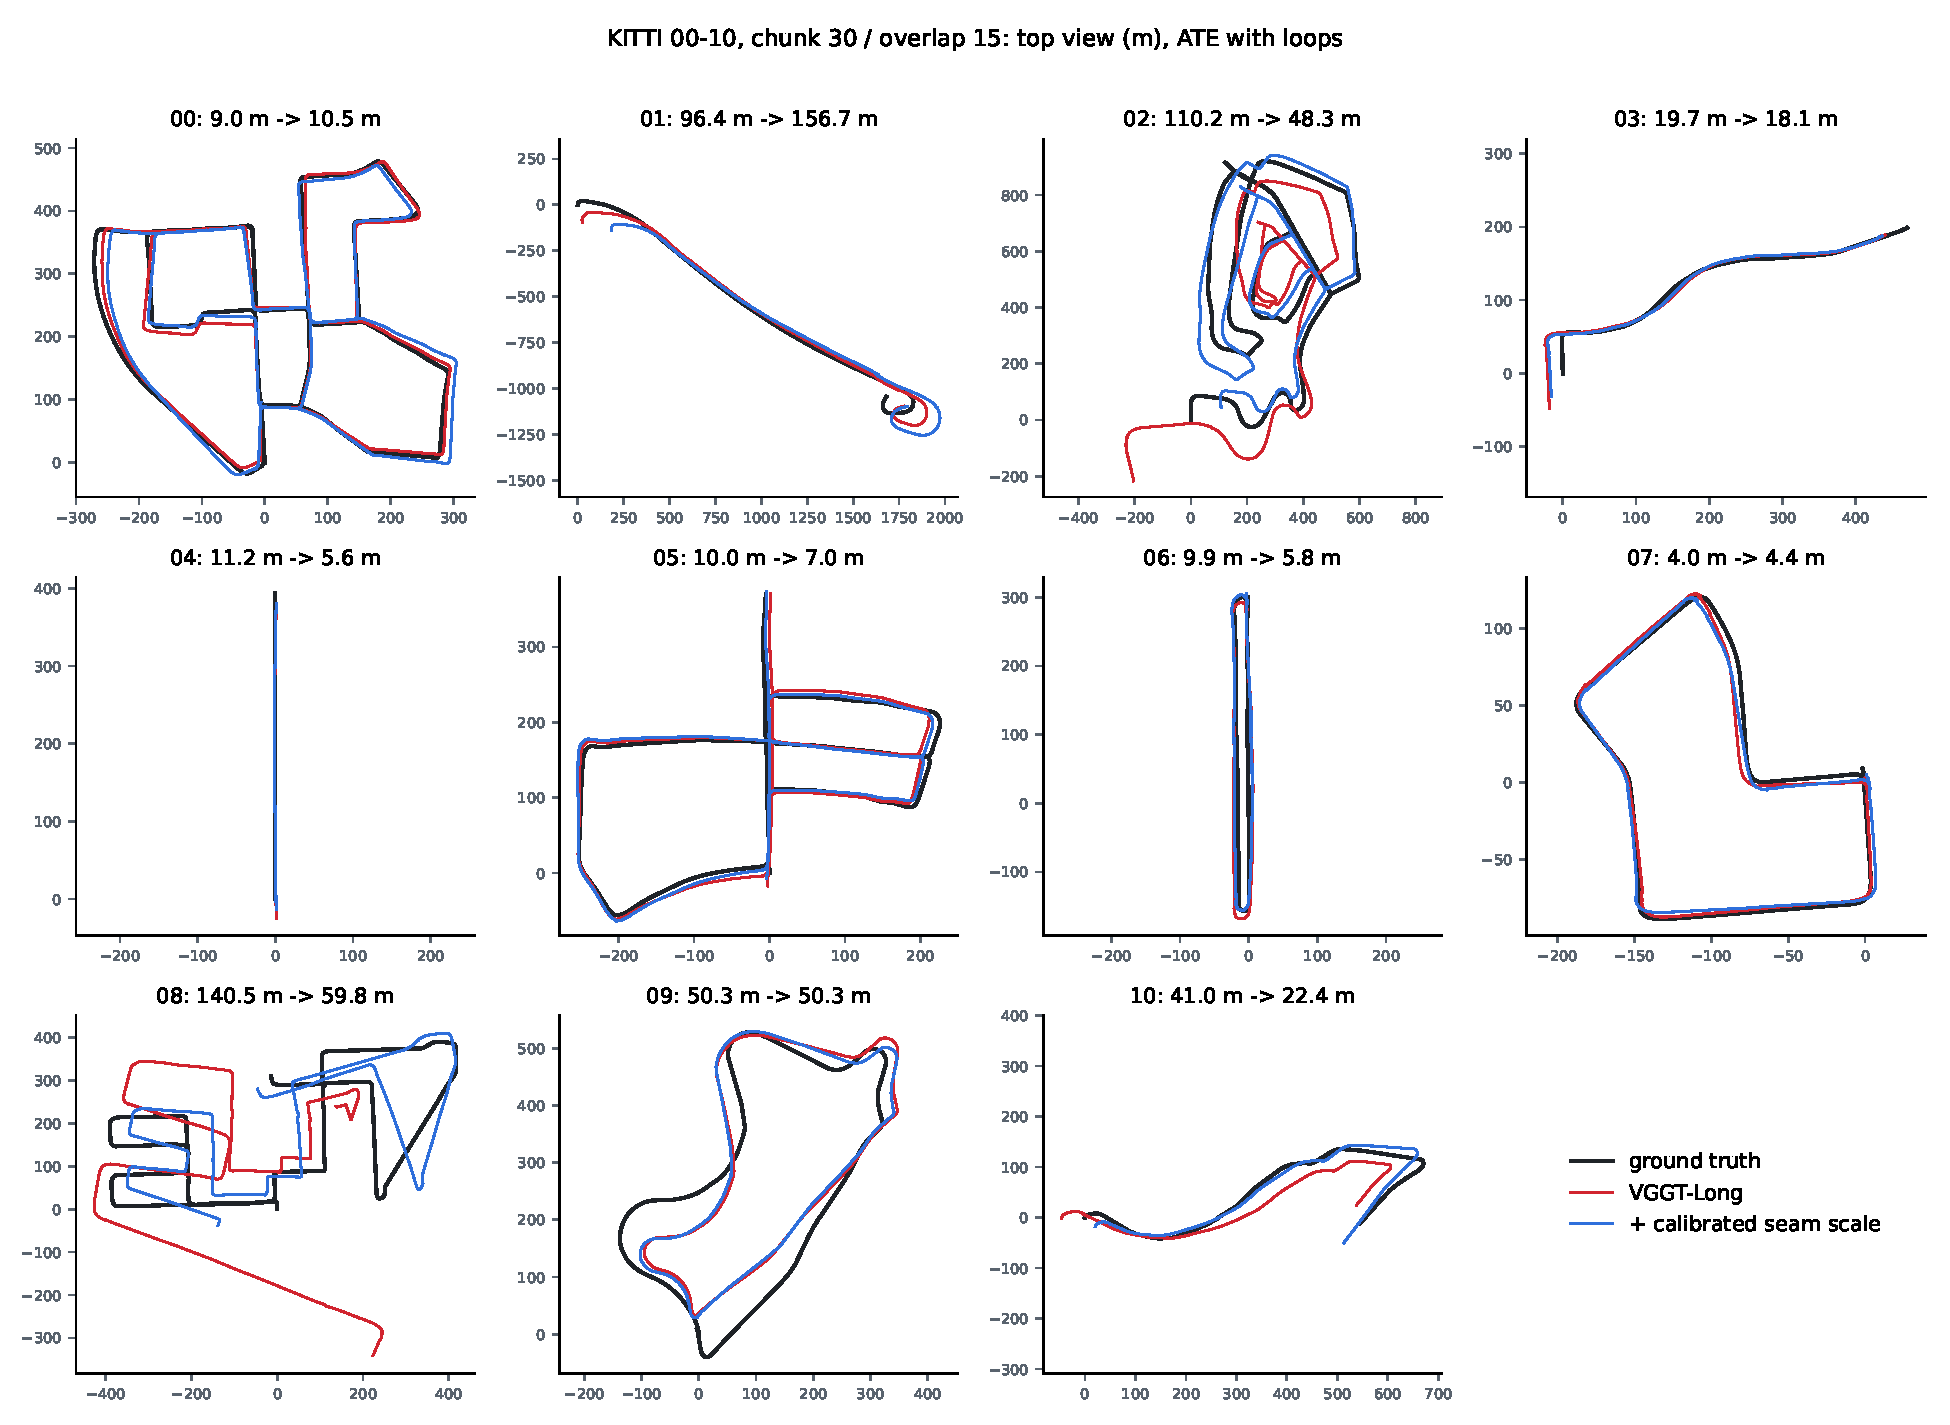
\includegraphics[width=0.80\textwidth]{fig_traj_first_w30_o15.pdf}
\caption{All eleven drives at 30/15 in our back end, with loops: ground truth, VGGT-Long, and VGGT-Long with the
calibrated seam scale (C4), after Sim(3) alignment. Panel titles give the ATE before and after.}
\label{fig:traj}
\end{figure}

\begin{table}[!h]
\centering
\caption{ATE (m) per drive in our back end at 60/30 and 75/30, loops on, every correction fitted on the other ten drives.}
\label{tab:big}
\footnotesize
\begin{tabular}{llrrrrrrrrrrrr}
\toprule
& & 00 & 01 & 02 & 03 & 04 & 05 & 06 & 07 & 08 & 09 & 10 & mean \\
\midrule
\multirow{5}{*}{60/30} & VGGT-Long & 8.54 & 57.18 & 54.61 & 8.98 & 4.46 & 9.09 & 4.63 & 2.68 & 74.29 & 31.79 & 27.80 & 25.82 \\
& + constant (C1) & 8.54 & 79.03 & 48.68 & 5.54 & 3.30 & 9.04 & 4.72 & 2.58 & 50.19 & 31.97 & 20.40 & 24.00 \\
& + calibrated scale (C4) & 8.85 & 86.34 & 50.67 & 15.57 & 2.20 & 5.35 & 3.24 & 1.80 & 51.47 & 28.39 & 12.52 & 24.22 \\
& + nested choice & 8.85 & 98.43 & 51.33 & 15.57 & 2.18 & 5.32 & 3.01 & 2.18 & 46.82 & 28.39 & 12.96 & 25.00 \\
& true scale & 8.24 & 27.59 & 41.17 & 3.09 & 0.82 & 3.70 & 2.85 & 2.30 & 40.91 & 17.39 & 10.04 & 14.37 \\
\midrule
\multirow{5}{*}{75/30} & VGGT-Long & 10.38 & 64.82 & 56.50 & 5.61 & 3.88 & 9.20 & 6.34 & 2.74 & 58.71 & 29.95 & 22.59 & 24.61 \\
& + constant (C1) & 10.38 & 77.95 & 51.46 & 6.38 & 3.20 & 9.22 & 6.52 & 2.68 & 48.89 & 30.10 & 18.32 & 24.10 \\
& + calibrated scale (C4) & 8.59 & 92.18 & 46.51 & 12.11 & 1.92 & 5.69 & 3.82 & 3.26 & 51.94 & 26.26 & 11.67 & 23.99 \\
& + nested choice & 8.41 & 103.97 & 51.82 & 10.76 & 2.10 & 5.94 & 4.22 & 1.85 & 49.40 & 28.70 & 11.91 & 25.37 \\
& true scale & 7.74 & 24.38 & 45.79 & 3.26 & 0.88 & 4.02 & 2.82 & 1.84 & 43.44 & 17.40 & 12.08 & 14.88 \\
\bottomrule
\end{tabular}
\end{table}

\begin{figure}[!h]
\centering
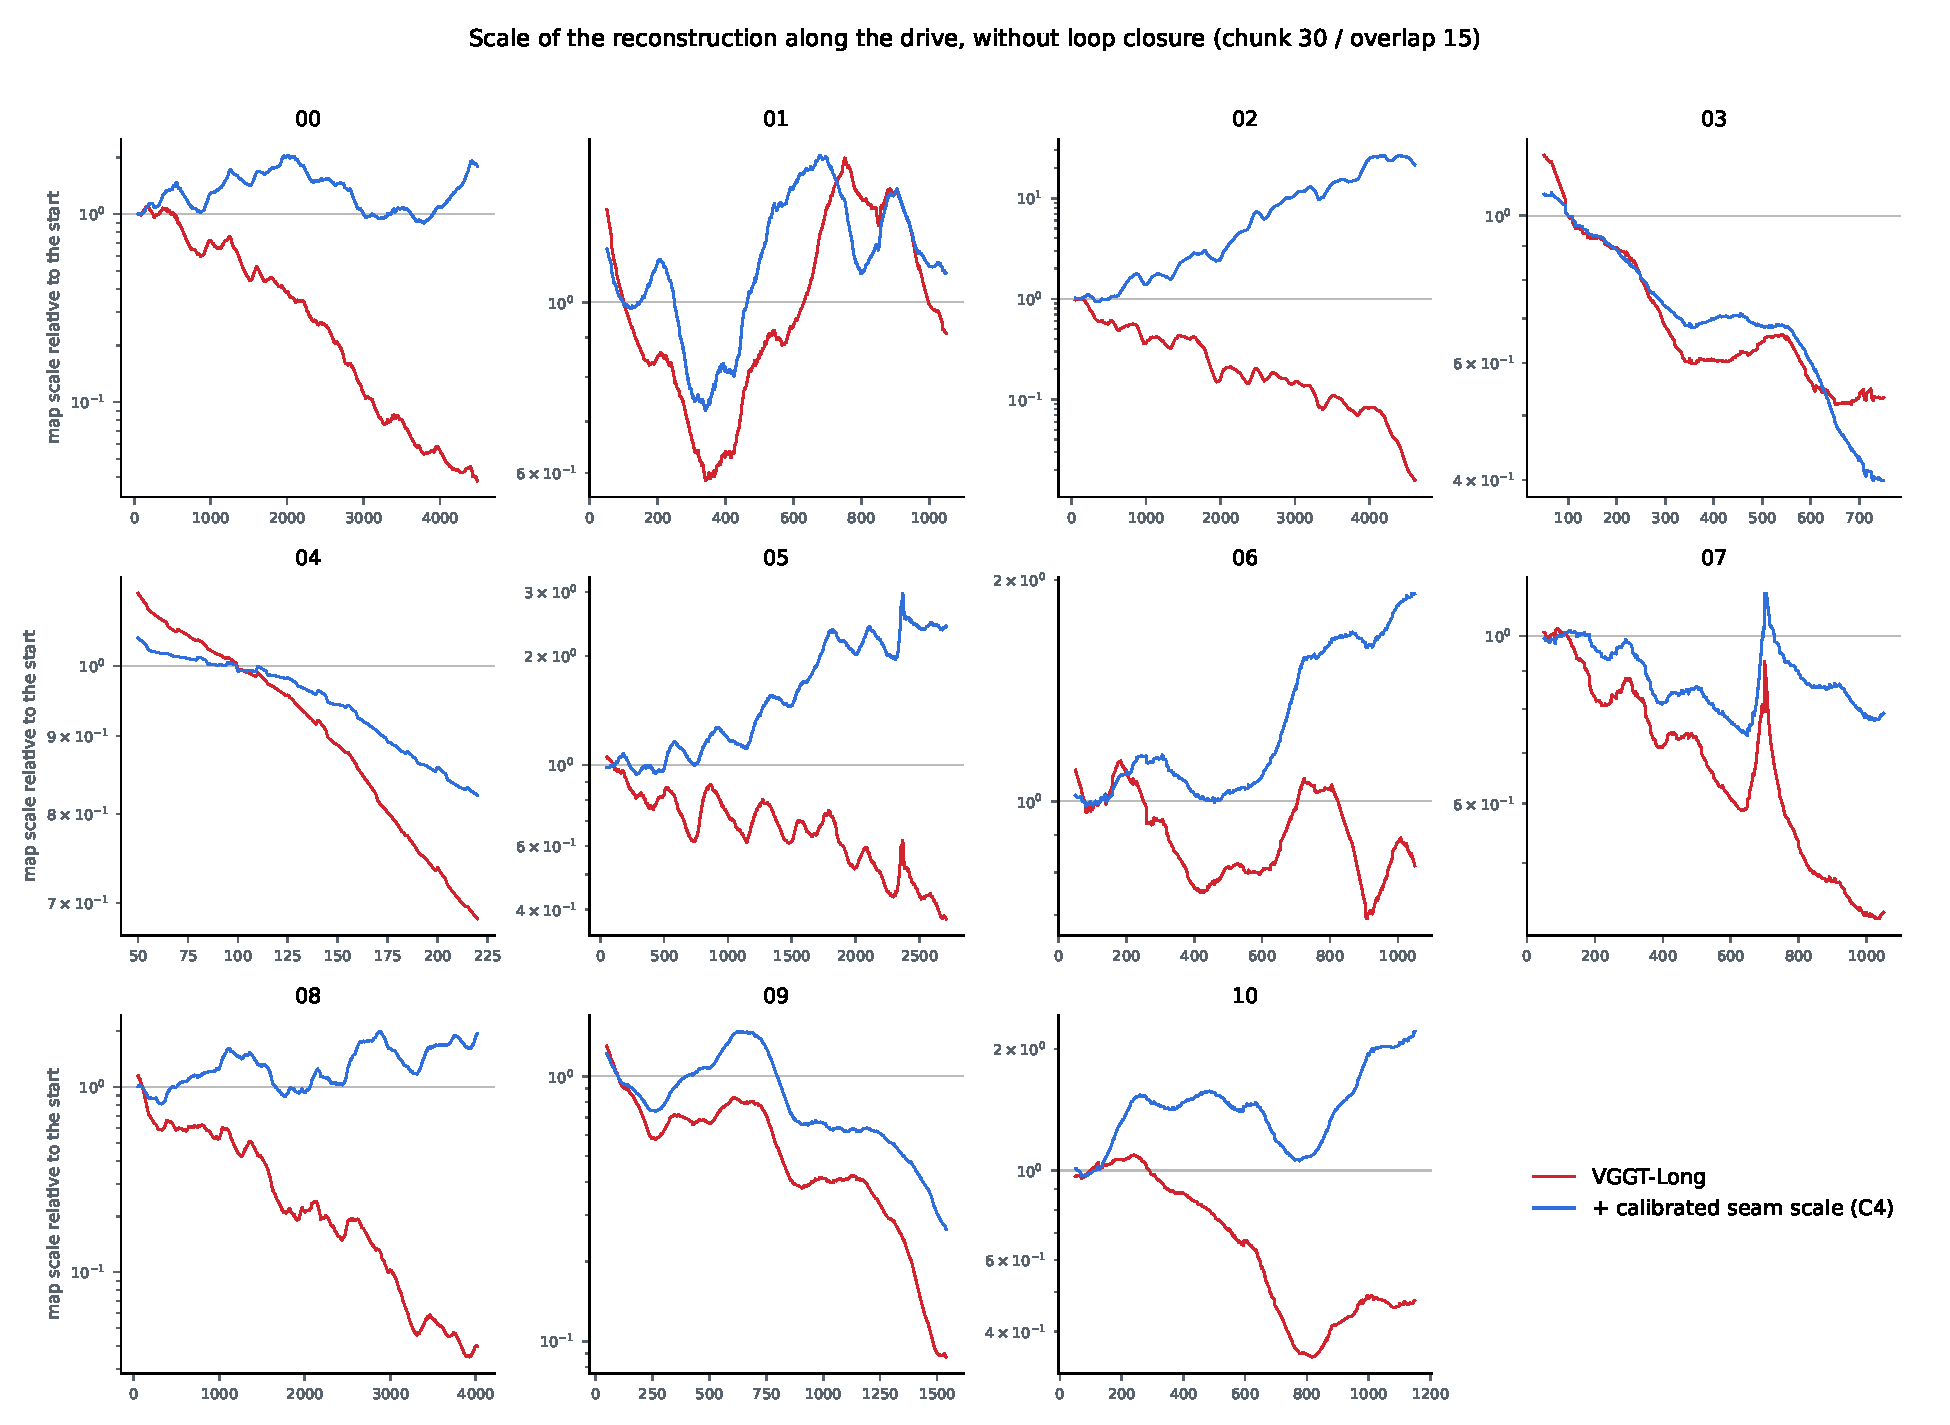
\includegraphics[width=0.80\textwidth]{fig_drift_first_w30_o15.pdf}
\caption{Scale of the reconstruction along each drive without loop closure, at 30/15: travelled distance of the estimate
over that of the ground truth in a sliding window of 100 frames, normalised to the start of the drive (1 = no drift).
VGGT-Long's map shrinks steadily on the long drives; the calibrated seam scale (C4) removes most of the shrinking but
can overshoot (02).}
\label{fig:drift}
\end{figure}

\begin{figure}[!h]
\centering
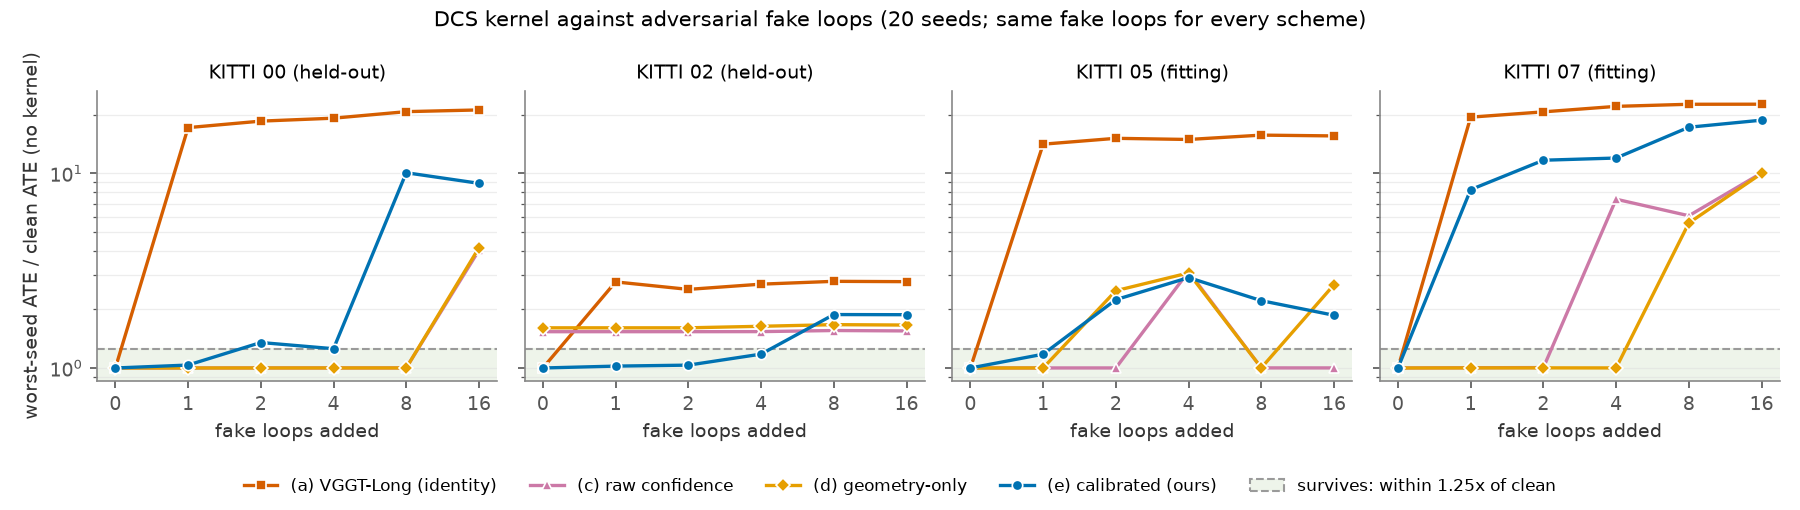
\includegraphics[width=0.92\textwidth]{stress_ratio_vs_fake_loops_w30.png}
\caption{False loops (window 30/15, DCS): worst ATE over 20 seeds relative to the clean graph without a kernel, against
the number of false loops added. The shaded band (within 1.25 times the clean graph) counts as surviving. Legend: (a) equal
weights as in VGGT-Long, (c) raw confidence, (d) geometry, (e) calibrated confidence. Equal weights fail with a single
false loop on every drive.}
\label{fig:stress}
\end{figure}

\end{document}
